%!TeX root=../wowtop.tex

\ArtChapter[At the Window]{11head}

\lettrine[lines=4,findent=2pt]{I}{} have already said that my storms of emotion have a trick of exhausting themselves. After a time I discovered that I was cold and wet, and with little pools of water about me on the stair carpet. I got up almost mechanically, went into the dining room and drank some whisky, and then I was moved to change my clothes.

After I had done that I went upstairs to my study, but why I did so I do not know. The window of my study looks over the trees and the railway towards Horsell Common. In the hurry of our departure this window had been left open. The passage was dark, and, by contrast with the picture the window frame enclosed, the side of the room seemed impenetrably dark. I stopped short in the doorway.

The thunderstorm had passed. The towers of the Oriental College and the pine trees about it had gone, and very far away, lit by a vivid red glare, the common about the sand-pits was visible. Across the light huge black shapes, grotesque and strange, moved busily to and fro.

It seemed indeed as if the whole country in that direction was on fire—a broad hillside set with minute tongues of flame, swaying and writhing with the gusts of the dying storm, and throwing a red reflection upon the cloud scud above. Every now and then a haze of smoke from some nearer conflagration drove across the window and hid the Martian shapes. I could not see what they were doing, nor the clear form of them, nor recognise the black objects they were busied upon. Neither could I see the nearer fire, though the reflections of it danced on the wall and ceiling of the study. A sharp, resinous tang of burning was in the air.

I closed the door noiselessly and crept towards the window. As I did so, the view opened out until, on the one hand, it reached to the houses about Woking station, and on the other to the charred and blackened pine woods of Byfleet. There was a light down below the hill, on the railway, near the arch, and several of the houses along the Maybury road and the streets near the station were glowing ruins. The light upon the railway puzzled me at first; there were a black heap and a vivid glare, and to the right of that a row of yellow oblongs. Then I perceived this was a wrecked train, the fore part smashed and on fire, the hinder carriages still upon the rails.

Between these three main centres of light—the houses, the train, and the burning county towards Chobham—stretched irregular patches of dark country, broken here and there by intervals of dimly glowing and smoking ground. It was the strangest spectacle, that black expanse set with fire. It reminded me, more than anything else, of the Potteries at night. At first I could distinguish no people at all, though I peered intently for them. Later I saw against the light of Woking station a number of black figures hurrying one after the other across the line.

And this was the little world in which I had been living securely for years, this fiery chaos! What had happened in the last seven hours I still did not know; nor did I know, though I was beginning to guess, the relation between these mechanical colossi and the sluggish lumps I had seen disgorged from the cylinder. With a queer feeling of impersonal interest I turned my desk chair to the window, sat down, and stared at the blackened country, and particularly at the three gigantic black things that were going to and fro in the glare about the sand-pits.

They seemed amazingly busy. I began to ask myself what they could be. Were they intelligent mechanisms? Such a thing I felt was impossible. Or did a Martian sit within each, ruling, directing, using, much as a man's brain sits and rules in his body? I began to compare the things to human machines, to ask myself for the first time in my life how an ironclad or a steam engine would seem to an intelligent lower animal.

The storm had left the sky clear, and over the smoke of the burning land the little fading pinpoint of Mars was dropping into the west, when a soldier came into my garden. I heard a slight scraping at the fence, and rousing myself from the lethargy that had fallen upon me, I looked down and saw him dimly, clambering over the palings. At the sight of another human being my torpor passed, and I leaned out of the window eagerly.

»Hist!« said I, in a whisper.

He stopped astride of the fence in doubt. Then he came over and across the lawn to the corner of the house. He bent down and stepped softly.

»Who's there?« he said, also whispering, standing under the window and peering up.

»Where are you going?« I asked.

»God knows.«

»Are you trying to hide?«

»That's it.«

»Come into the house,« I said.

I went down, unfastened the door, and let him in, and locked the door again. I could not see his face. He was hatless, and his coat was unbuttoned.

»My God!« he said, as I drew him in.

»What has happened?« I asked.

»What hasn't?« In the obscurity I could see he made a gesture of despair. »They wiped us out—simply wiped us out,« he repeated again and again.

He followed me, almost mechanically, into the dining room.

»Take some whisky,« I said, pouring out a stiff dose.

He drank it. Then abruptly he sat down before the table, put his head on his arms, and began to sob and weep like a little boy, in a perfect passion of emotion, while I, with a curious forgetfulness of my own recent despair, stood beside him, wondering.

It was a long time before he could steady his nerves to answer my questions, and then he answered perplexingly and brokenly. He was a driver in the artillery, and had only come into action about seven. At that time firing was going on across the common, and it was said the first party of Martians were crawling slowly towards their second cylinder under cover of a metal shield.

Later this shield staggered up on tripod legs and became the first of the fighting-machines I had seen. The gun he drove had been unlimbered near Horsell, in order to command the sand-pits, and its arrival it was that had precipitated the action. As the limber gunners went to the rear, his horse trod in a rabbit hole and came down, throwing him into a depression of the ground. At the same moment the gun exploded behind him, the ammunition blew up, there was fire all about him, and he found himself lying under a heap of charred dead men and dead horses.

% \begin{figure}[tbp]
% \centering
% 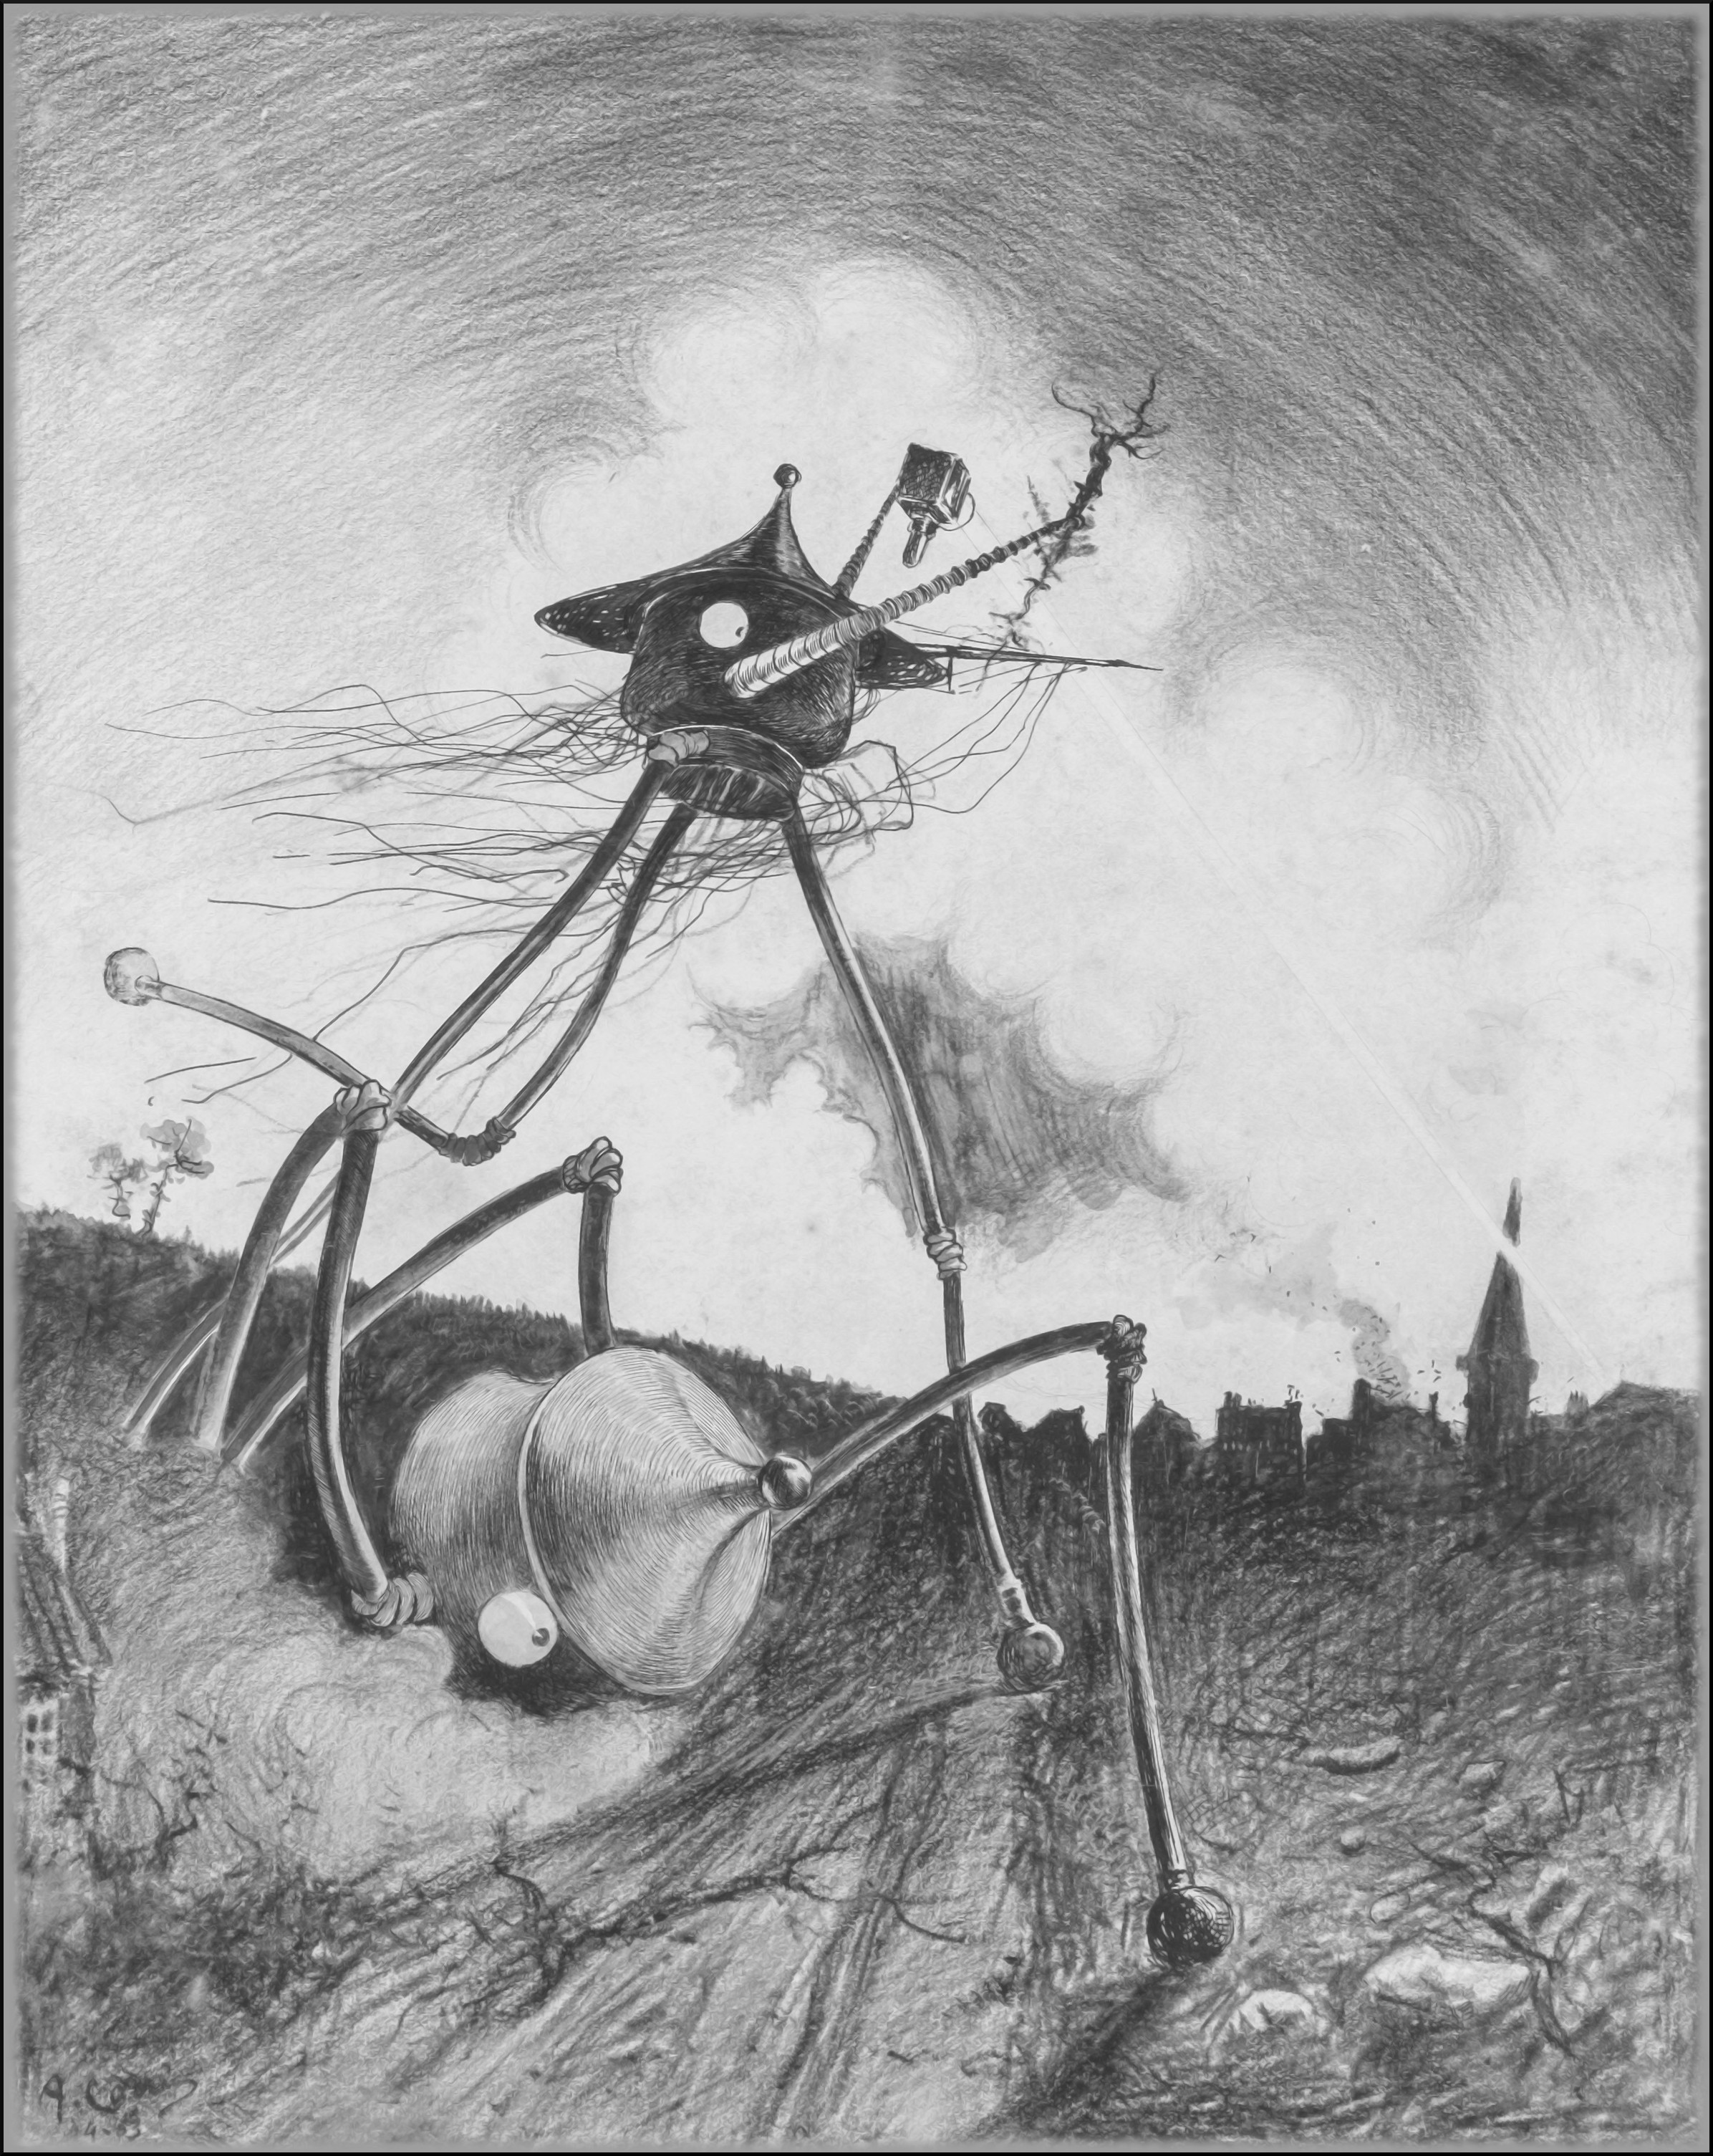
\includegraphics[width=\linewidth]{11shield}
% \caption{This shield staggered up on tripod legs}
% \end{figure}

\begin{bwbigpic}
	[1.2] 
	{11shield} 
	{This shield staggered up on tripod legs} 
\end{bwbigpic}

»I lay still,« he said, »scared out of my wits, with the fore quarter of a horse atop of me. We'd been wiped out. And the smell—good God! Like burnt meat! I was hurt across the back by the fall of the horse, and there I had to lie until I felt better. Just like parade it had been a minute before—then stumble, bang, swish!«

»Wiped out!« he said.

He had hid under the dead horse for a long time, peeping out furtively across the common. The Cardigan men had tried a rush, in skirmishing order, at the pit, simply to be swept out of existence. Then the monster had risen to its feet and had begun to walk leisurely to and fro across the common among the few fugitives, with its headlike hood turning about exactly like the head of a cowled human being. A kind of arm carried a complicated metallic case, about which green flashes scintillated, and out of the funnel of this there smoked the Heat-Ray.

In a few minutes there was, so far as the soldier could see, not a living thing left upon the common, and every bush and tree upon it that was not already a blackened skeleton was burning. The hussars had been on the road beyond the curvature of the ground, and he saw nothing of them. He heard the Maxims rattle for a time and then become still. The giant saved Woking station and its cluster of houses until the last; then in a moment the Heat-Ray was brought to bear, and the town became a heap of fiery ruins. Then the Thing shut off the Heat-Ray, and turning its back upon the artilleryman, began to waddle away towards the smouldering pine woods that sheltered the second cylinder. As it did so a second glittering Titan built itself up out of the pit.

The second monster followed the first, and at that the artilleryman began to crawl very cautiously across the hot heather ash towards Horsell. He managed to get alive into the ditch by the side of the road, and so escaped to Woking. There his story became ejaculatory. The place was impassable. It seems there were a few people alive there, frantic for the most part and many burned and scalded. He was turned aside by the fire, and hid among some almost scorching heaps of broken wall as one of the Martian giants returned. He saw this one pursue a man, catch him up in one of its steely tentacles, and knock his head against the trunk of a pine tree. At last, after nightfall, the artilleryman made a rush for it and got over the railway embankment.

Since then he had been skulking along towards Maybury, in the hope of getting out of danger Londonward. People were hiding in trenches and cellars, and many of the survivors had made off towards Woking village and Send. He had been consumed with thirst until he found one of the water mains near the railway arch smashed, and the water bubbling out like a spring upon the road.

\begin{figure}[tb]
\centering

\includegraphics[width=\linewidth]{11chat}
\end{figure}

That was the story I got from him, bit by bit. He grew calmer telling me and trying to make me see the things he had seen. He had eaten no food since midday, he told me early in his narrative, and I found some mutton and bread in the pantry and brought it into the room. We lit no lamp for fear of attracting the Martians, and ever and again our hands would touch upon bread or meat. As he talked, things about us came darkly out of the darkness, and the trampled bushes and broken rose trees outside the window grew distinct. It would seem that a number of men or animals had rushed across the lawn. I began to see his face, blackened and haggard, as no doubt mine was also.

\begin{wrapfigure}{O}{0.5\textwidth}
\centering

\includegraphics[width=0.5\textwidth]{11tailpiece}
\end{wrapfigure}

When we had finished eating we went softly upstairs to my study, and I looked again out of the open window. In one night the valley had become a valley of ashes. The fires had dwindled now. Where flames had been there were now streamers of smoke; but the countless ruins of shattered and gutted houses and blasted and blackened trees that the night had hidden stood out now gaunt and terrible in the pitiless light of dawn. Yet here and there some object had had the luck to escape—a white railway signal here, the end of a greenhouse there, white and fresh amid the wreckage. Never before in the history of warfare had destruction been so indiscriminate and so universal. And shining with the growing light of the east, three of the metallic giants stood about the pit, their cowls rotating as though they were surveying the desolation they had made.

It seemed to me that the pit had been enlarged, and ever and again puffs of vivid green vapour streamed up and out of it towards the brightening dawn—streamed up, whirled, broke, and vanished.

Beyond were the pillars of fire about Chobham. They became pillars of bloodshot smoke at the first touch of day.

%\begin{figure}[b!]
%\centering
%
\includegraphics[width=0.7\textwidth]{11tailpiece}\captionlistentry{Tailpiece to Chapter \thechapter}
%\end{figure}